\documentclass{article}
\usepackage{hyperref}
\usepackage{graphicx}
\usepackage{tabularx}
\usepackage{amsmath}
\usepackage{multirow}
\usepackage{subcaption}

\title{Protecting against Knowledge Poisoning Attacks}
\author{Ollie Matthews}
\date{}

\begin{document}

\maketitle

\begin{abstract}
This paper presents an investigation of defenses against knowledge poisoning attacks, as described in the "PoisonedRAG" paper. It explores different mitigation strategies aimed at reducing the number of poisoned answers to questions. The results show that the risk of these attacks can be largely mitigated with a combination of chain-of-thought (CoT) prompting, a "danger evaluation" model, and encouraging variance in the retrieved results. The paper also discusses the limitations of other approaches and the importance of this research in the context of building robust language model-based systems.
\end{abstract}

\section{Introduction}

Retrieval-Augmented Generation (RAG) systems can be a useful way of increasing the useful information output of Large Language Models (LLMs) by giving them access to information not included in their training data. However, giving RAG systems direct access to potentially untrusted data can open up new vulnerabilities. 

In the "PoisonedRAG" paper \cite{zou2024poisonedrag}, it is shown that someone with access to the RAG corpus can inject texts which will be picked up by the retriever. These texts can make the model output an incorrect answer to a question. It has also been shown that prompt injections can be indirectly included via data retrieval \cite{greshake2023youve}. 

This paper investigates different ways to mitigate against these attacks with the goal of reducing the number of poisoned answers to questions. 

\section{Method}

The poisoned contexts generated in the PoisonedRAG paper are used in this study. The study is evaluated on the "nq" dataset, although extension to the other datasets in the RAG paper would be simple with more time. 

The general pipeline is as follows:

\begin{itemize}
\item A set of 100 questions from the nq dataset for which the PoisonedRAG paper has generated five poisoned context items each is used.
\item An extended corpus is created which has the standard nq corpus, as well as all of the poisoned context items.
\item For each context item in the extended corpus, OpenAI's "text-embedding-3-small" model is used to generate an embedding.
\item For a given question, the $n$ closest contexts (in cosine similarity) to the embedding of the question are retrieved. If not specified otherwise, $n$ is set to 5.
\item The question is then answered, using the retrieved contexts. An answer is "correct" if the correct answer appears in the output of the LLM. An answer is "poisoned" if the target "poisoned" answer appears in the output of the LLM.
\item The primary interest is in the percentage of poisoned answers.
\end{itemize}

This process is conducted with both `gpt3.5-turbo` and `gpt-4o`.

\section{Mitigations}

To mitigate against the risks from the LLM, the following techniques are used:

\begin{itemize}
\item \textbf{Prompt Tuning (Refined Prompt):} The prompt in the original "PoisonedRAG" paper tells the LLM to respond to the user's question, and that there is "context to help [the llm] answer". This is addressed in a "refined" prompt by emphasizing the LLM should respond "truthfully", emphasizing that the contexts are not trusted, and could be misleading, and telling the LLM to simply ignore any context which is not true, or talks about a hypothetical situation which is not relevant.
\item \textbf{CoT Prompting:} This technique supplements the "refined" prompt strategy with CoT prompting. The LLM is told it must give "Reasoning" for its answer, and then answer afterwards. Examples of responses, including those that show poisoned contexts, are also provided.
\item \textbf{Danger Evaluator (DE):} A separate instance of the LLM is used to evaluate contexts before passing them to the response LLM. This "Danger Evaluator" LLM is told to look out for inconsistencies between the contexts, false information in the contexts, contexts which refer to a hypothetical situation, and contexts which contain prompt injections.
\item \textbf{Context Variance Encouragement (CVE):} A "variance encouragement" step is added to the context retrieval process. This is aimed at encouraging sources which provide varied information (and a different point of view).
\end{itemize}

\section{Results}

\section{Results}

\subsection{Main Results}

The main results showing the "PoisonedRAG Success Rate" are illustrated in Figure~\ref{fig: main_plot}. This denotes the number of responses that were successfully "poisoned" by the PoisonedRAG attack. The mitigations introduced significantly lower the success rate of PoisonedRAG for both models.

\begin{figure}[h!]
\centering
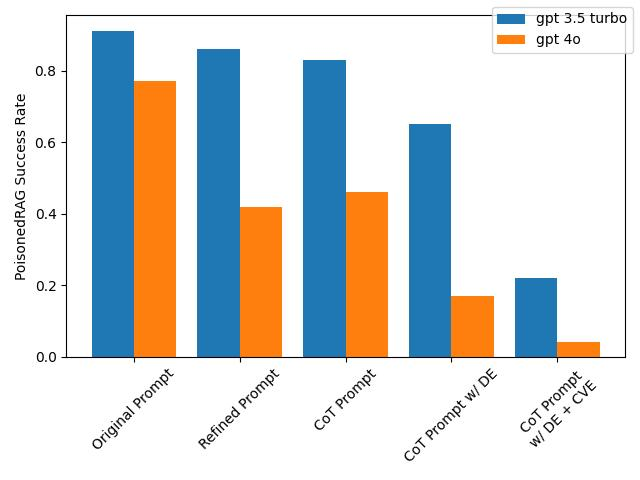
\includegraphics[width=0.5\textwidth]{../figures/main_plot.jpg}
\caption{Main Results}
\label{fig: main_plot}
\end{figure}

\subsubsection{Refined Prompt}

Refining the prompt dramatically decreases the attack success rate, especially with the more potent `gpt-4o`. By tuning the LLM to disregard hypothetical situations, `gpt-4o` correctly provides the factual answer against the poisoned one, though `gpt-3.5-turbo` fails to do so.

\subsubsection{CoT Prompting}

The efficiency of `gpt3.5` significantly improves because of CoT prompting, as noted in previous studies~\cite{DBLP:journals/corr/abs-2201-11903}, while the effect on `gpt-4o` is minimal.

\subsubsection{Danger Evaluator}

Adding a separate "Danger Evaluator" remarkably magnifies performance. The evaluator identifies higher danger rates "individually" rather than "combined" (refer Table ~\ref{tbl:rates}). Even though a single LLM should be capable of identifying threats and react accordingly, this indicates that LLMs perform better when tasked with smaller, more focused operations.

\begin{table}[h!]
\centering
\begin{tabular}{|c|c|c|c|}
\hline
\multirow{2}{*}{Context Pipeline} & \multirow{2}{*}{Danger Evaluator} & \multicolumn{2}{c|}{Danger Evaluation Rate}\\
\cline{3-4}
 & & DIR (gpt-3.5-turbo) & DIR (gpt-4o)\\
\hline
\multirow{2}{*}{No CVE} & Combined & 0.19 & 0.73\\
 & Individual & 0.34 & 0.83\\
\hline
\multirow{2}{*}{With CVE} & Combined & 0.11 & 0.93\\
 & Individual & 0.53 & 0.95\\
\hline
\end{tabular}
\caption{Danger Evaluation Rates}
\label{tbl:rates}
\end{table}

\subsubsection{Danger Evaluator with Context Variance Encouragement}

Data indicates that Context Variance Encouragement enhances robustness to attacks. With CVE, the "Danger Evaluator" correctly identifies 95\% of attacks when used with `gpt-4o`. This approach protects against many-shot jailbreak type attacks by limiting the effect of false information and the LLM's inability to handle many similar contexts.

\paragraph{Performance with varying number of poisoned texts}
The impact of increasing the number of poisoned texts on the pipeline is demonstrated below in Figure~\ref{fig: poison_eval}. It shows that the performance drops as the number of poisoned items increase, indicating the difficulty for even the more potent `gpt-4o` model to identify contradictions in the context. However, the use of Context Variance Encouragement mitigates this effect to a considerable extent. 

\begin{figure}[h!]
  \centering
  \begin{subfigure}[b]{0.45\textwidth}
    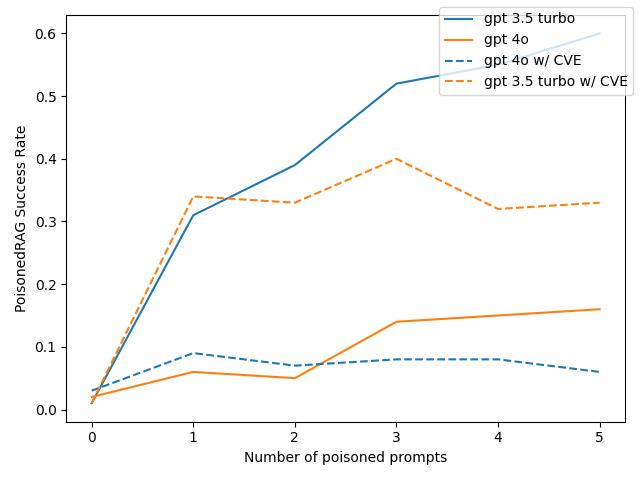
\includegraphics[width=\textwidth]{../figures/varying_n_poisoned.jpg}
    \caption{Varying number of poisoned texts}
  \end{subfigure}
  \begin{subfigure}[b]{0.45\textwidth}
    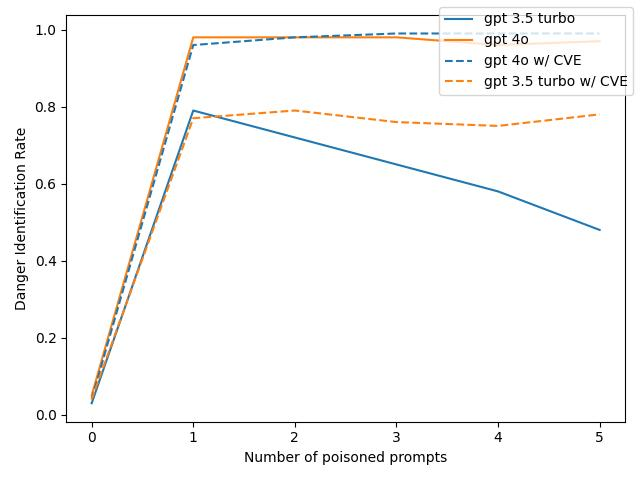
\includegraphics[width=\textwidth]{../figures/varying_n_dangerous_eval.jpg}
    \caption{Danger Evaluator's performance with varying number of poisoned texts}
  \end{subfigure}
  \caption{Performance with varying number of poisoned texts}
  \label{fig: poison_eval}
\end{figure}

\section{Conclusion}

This project suggests a pipeline for making RAG systems more robust to attacks similar to the PoisonedRAG paper. The final approach is able to defend against Poisoned RAG attacks 96\% of the time with `gpt-4o`, and 78\% of the time with `gpt-3.5-turbo`. Some limitations remain, but the suggested mitigations could make it much easier to deploy RAG systems in safety. 

\bibliographystyle{plain}
\bibliography{references}

\end{document}
